\documentclass{article}
\usepackage{graphicx} % Required for inserting images
\usepackage{chemfig}
\usepackage{chemformula}
\usepackage[version=4]{mhchem}
\usepackage{modiagram}
\usepackage{multirow}
\usepackage{amsmath}
\usepackage{lewis}
\graphicspath{ {./photos/} }

\title{Monopoly Problems}
\author{Andrew Ye and Diva Shah}
\date{May 2024}

\begin{document}
\maketitle
\newpage
\tableofcontents
\newpage

\section{Unit 1: Atomic Structure and Properties}
\subsection*{Problem 1}
Calculate the number of moles in a \(7.89 kg\) sample of \(\ce{C_9H_8O_4}\) 
\subsection*{Problem 2}
Given this graph, what is true about the element depicted
\begin{center}
    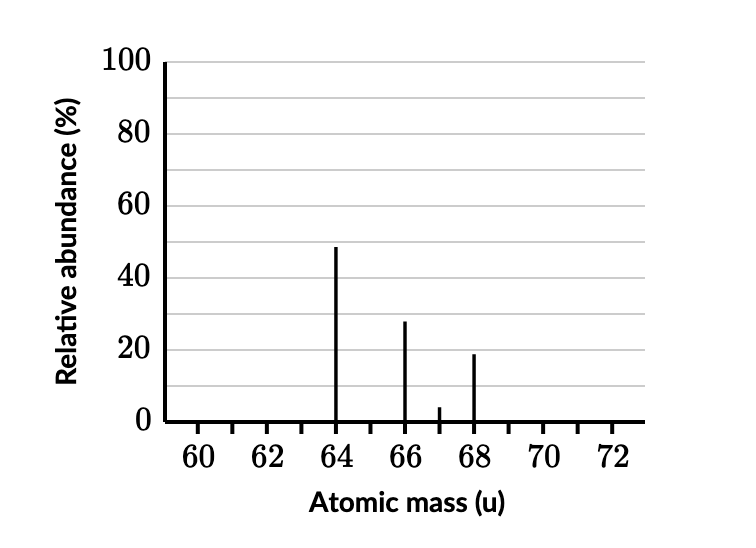
\includegraphics[scale = 0.5]{photos/photo1.png}
\end{center}
(a) In an average sample of the element, less than \(20\%\) of the atoms have an atomic mass of \(66u\). \\
(b) The most abundant isotope of the element has an atomic mass of \(64u\). \\
(c) The element has an average atomic mass of \(64u\). \\
(d) The element has an average atomic mass between \(66\) and \(68u\). \\
\subsection*{Problem 3}
What is the percent composition of Carbon in \(\ce{C_{13}H_{18}O_2}\)?
\subsection*{Problem 4}
A compound contains \(32.38\%\) sodium, \(22.65\%\) sulfur, and \(44.99\%\) oxygen. What is the emperical forumula. 
\subsection*{Problem 5}
What is the full electron configuration of mercury?
\subsection*{Problem 6}
Below, the photoelectron spectra of the \(2s\) electrons of \(\ce{Be}\) and \(\ce{Mg}\) are shown.
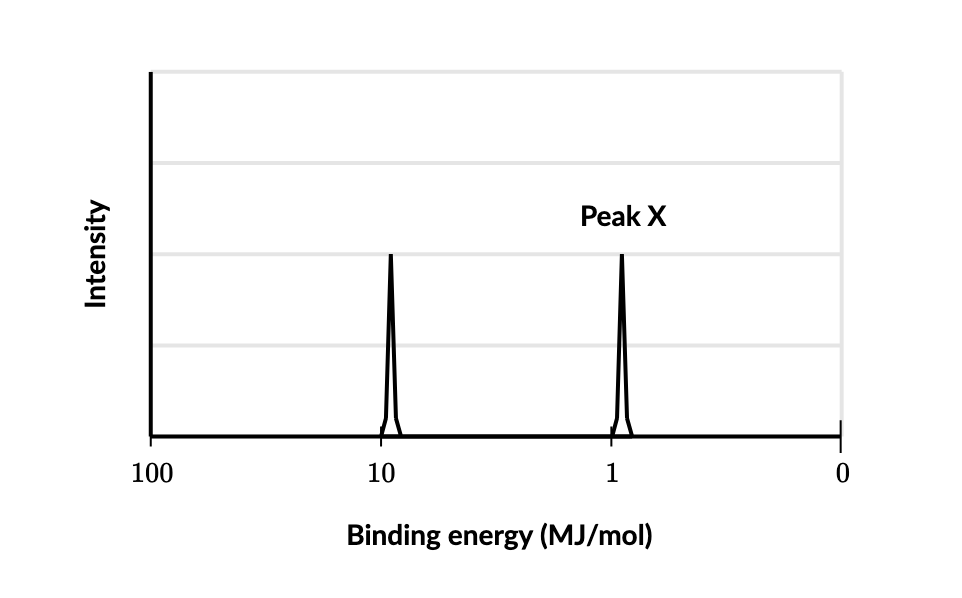
\includegraphics[scale = 0.5]{photos/photo2.png} \\
Is peak \(X\) the peak associated with \(\ce{Be}\) or \(\ce{Mg}\)?



\newpage
\section{Answers}
\subsection{Unit 1}
\subsubsection*{Problem 1}
The molar mass of \(\ce{C_9H_8O_4}\) is \(1.008*8 + 12.01*9 + 16.00*4 = 180.2 \frac{g}{mol}\)
\begin{equation}
\begin{aligned}
    7.89kg \times \frac{1g}{10^{-3}kg} \times \frac{1mol}{180.2g} = 43.8mol
\end{aligned}
\end{equation}
\subsubsection*{Problem 2}
(b), the tallest peak of the graph is the one at \(64u\). 
\subsubsection*{Problem 3}
In one mole of \(\ce{C_{13}H_{18}O_2}\) is \(206.31g\).
\begin{equation}
\begin{aligned}
    1mol\hspace{0.1em}\ce{C_{13}H_{18}O_2} \times \frac{13mol\hspace{0.1em}\ce{C}}{1mol\ce{C_{13}H_{18}O_2}} \times \frac{12.01g}{1mol\hspace{0.1em}\ce{C}} = 156.31g
\end{aligned}
\end{equation}
Thus, the percent composition by weight is \(\frac{156.31}{206.31} = 75.764\%\)
\subsubsection*{Problem 4}
Take \(100g\) of the substance such that there are \(32.38g\) sodium, \(22.65g\) sulfur, and \(44.99g\) oxygen. 
\begin{equation}
\begin{aligned}
    32.38g\hspace{0.1em}\ce{Na} \times \frac{1mol\hspace{0.1em}\ce{Na}}{22.99g} &= 1.408mol\hspace{0.1em}\ce{Na} \\
    22.65\hspace{0.2em}g \ce{S} * \frac{1\hspace{0.2em}mol\ce{S}}{32.07g} &= 0.7063 \hspace{0.2em}mol\ce{S}\\
    44.99\hspace{0.2em}g\ce{O} * \frac{1\hspace{0.2em}mol\ce{O}}{16 g} &= 2.812\hspace{0.2em}mol \ce{O}
\end{aligned}
\end{equation}
Take the ratio of each compound with the smallest quantity. 
\begin{equation}
\begin{split}
    S:\hspace{0.2em}\frac{0.7063}{0.7063} = 1 \\
    Na:\hspace{0.2em}\frac{1.408}{0.7063} = 2 \\
    O:\hspace{0.2em}\frac{2.812}{0.7063} = 4
\end{split}
\end{equation}
Therefore, the empirical formula is \(Na_{2}SO_{4}\)
\subsubsection*{Problem 5}
\(1s^22s^22p^63s^23p^64s^23d^{10}4p^65s^24d^{10}5p^66s^24f^{14}5d^{10}\)
\subsubsection*{Problem 6}
\(\ce{Be}\). The peak location of the peak on the x-axis means that there is less binding energy for the electrons in element \(X\). \(\ce{Be}\) has fewer protons
and both electrons are in the same shell, so it peak must belong to \(\ce{Be}\).

\end{document}